\documentclass[
    bachelor,
    blackurls,
    titleikn
]{mthesis}

%%%%%%%%%%%%%%%%%%%%%%%%%%%%%%%%%%%%%%%%%%%%%%%%%%%%%%%%%%%%%%%%%%%
% Параметры класса документа

%---------
% тип ВКР
%---------
% bachelor  - бакалаврская диссертация
% master    - магистерская диссертация

%-------------
% гиперссылки
%-------------
% blackurls - ссылки на литературу, таблицы, рисунки, формулы и т.п.
%             не выделяются цветом (используется для ч/б печати)
% colurls   - цветные ссылки (для распространения пояснительной записки 
%             в электронном виде)

%-----------------------------
% оформление титульного листа
%-----------------------------
% titlestd  - согласно методическим указаниям
% titleasu  - согласно требованиям ИКН


%%%%%%%%%%%%%%%%%%%%%%%%%%%%%%%%%%%%%%%%%%%%%%%%%%%%%%%%%%%%%%%%%%%%
% Здесь следует размещать допольнительные пакеты и команды. Следующие 
% пакеты уже загружены в стилевой файл: geometry, amssymb, mathtools, 
% ifthen, cmap, textcomp, babel, upgreek, indentfirst, xcolor, calc, 
% tabularray, icomma, ulem, soulutf8, tikz, hyperref, graphicx, 
% caption, subcaption, pdfpages, aliascnt, totalcount, totcount, 
% totpages, placeins, enumitem, biblatex, fancyvrb, listings

% например, для создания данного примера ВКР потребовались 
% следующие пакеты и команды:

% пакет для вёрстки сложных матриц
\usepackage{nicematrix}

% пакет для вставки примеров изображений
\usepackage{duckuments}

% пакет для оформления блоков цитирования
\usepackage{csquotes}

% пример команды, знак С++
\newcommand{\cpp}{%
    C\nolinebreak\hspace{-.05em}%
    \raisebox{.2ex}{+}\nolinebreak\hspace{-.10em}%
    \raisebox{.2ex}{+}%
}

% доп. библиотеки tikz
\usetikzlibrary{shapes.geometric, shapes.misc, arrows, positioning}

% стили tikz для рисования блок-схемы
\tikzset{
  line/.style = {thick},
  startstop/.style = {rounded rectangle, line, minimum width=3cm, 
    minimum height=1cm, text centered, draw=black, fill=white},
  io/.style = {trapezium, line, trapezium stretches=true, trapezium left angle=70, 
    trapezium right angle=110, minimum width=3cm, minimum height=1cm, 
    text centered, draw=black, fill=white},
  process/.style = {rectangle, line, minimum width=3cm, minimum height=1cm, 
    text centered, text width=3cm, draw=black, fill=white},
  decision/.style = {diamond, line, minimum width=3cm, minimum height=1cm, 
    text centered, draw=black, fill=white, aspect=2},
  arrow/.style = {line,->,>=stealth},
}


%%%%%%%%%%%%%%%%%%%%%%%%%%%%%%%%%%%%%%%%%%%%%%%%%%%%%%%%%%%%%%%%%%%%
% Информация для заполнения титульного листа и задания на ВКР

% ФИО студента
\AuthorShortName{Иванов И.И.}
\AuthorFullName{Иванов Иван Иванович} % полностью
\AuthorFullNameGen{Иванову Ивану Ивановичу} % полностью в родительном падеже
% Номер группы
\AuthorGroup{БИВТ-18-2}

% Тема работы
\ThesisTitle{Разработка и исследование алгоритмов искусственного 
интеллекта для обнаружения дефектов сверхпрочных термопластических 
материалов на изображениях высокого разрешения}

% Научный руководитель
\SupervisorShort{Петров П.П.}
\SupervisorFull{Петров Петр Петрович}
\SupervisorDegree{Доцент кафедры АСУ, к.т.н., доц.}

% Нормоконтроль
\GOSTComplianceReviewer{Смирнов С.С.}
% Проверка на заимствования
\PlagiarismChecker{Кузнецов К.К.}

% Название кафедры, ФИО зав. кафедрой
\DeptShort{АСУ}
\DeptFull{АВТОМАТИЗИРОВАННЫХ СИСТЕМ УПРАВЛЕНИЯ}
\DeptHead{Темкин И.О.}

% Название института, ФИО директора
\InstShort{ИТКН}
\InstFull{ИНФОРМАЦИОННЫХ ТЕХНОЛОГИЙ И КОМПЬЮТЕРНЫХ НАУК}
\InstHead{Солодов С.В.}

% Шифр специальности, краткое и полное наименование специальности
% 09.03.01 – это бакалавриат, а 09.04.01 – магистратура
\SpecShort{09.03.01 ИВТ}
\SpecFull{09.03.01 ИНФОРМАТИКА И ВЫЧИСЛИТЕЛЬНАЯ ТЕХНИКА}

% Место и год выполнения работы
\City{Москва}
\Year{2033}

% Цель работы
\ThesisPurpose{Повышение точности обнаружения дефектов углеродных волокон.}

% Исходные данные
\ThesisData{Изображения углеродных волокон высокого разрешения, 
полученные с помощью сканирующего электронного микроскопа.}
 
% Основная литература, в том числе:
% Монографии, учебники и т.п.
\ThesisBooks{%
1)~Goodfellow~I., Bengio~Y., Courville~A. Deep Learning. 
Cambridge, MA: MIT Press, 2016.~--- 800~p.;
2)~Hyndman R.J., Athanasopoulos G. 
Forecasting: Principles and Practice. 3rd ed. 
Melbourne, Australia: OTexts, 2021.~--- 442~p.;
3)~Неруш Ю.М., Панов С.А., Неруш А.Ю. Проектирование
логистических систем~--- М.:~Юрайт, 2016.~--- 408~с.}

% Отчеты по НИР, диссертации, дипломные работы и т.п.
\ThesisReports{%
1)~Зайцева Е.В. Разработка научно-методической базы обоснования 
и комплексного планирования стратегий развития горноперерабатывающих 
производств с учетом инновационной составляющей: дис. ... докт. техн. 
наук: 05.02.22.~--- МИСИС, Москва, 2020.~--- 329~с.;
2)~Колодин Е.Д. Динамическое построение маршрутов перемещения 
автономного транспорта в~карьерах: выпускная квалификационная работа
бакалавра: 09.03.01.~--- МИСИС, Москва, 2023.~--- 59~с.}

% Периодическая литература (журналы)
\ThesisJournals{%
1)~Умар~М.З., Вавилов~В.П., Абдулла~Х., Ариффин~А.К. 
Обнаружение низкоэнергетических ударных повреждений 
в углерод-углеродных композитах с~помощью ультразвуковой инфракрасной 
термографии //~Дефектоскопия.~--- 2017.~--- №~7.~--- С.~62--70;
2)~Cook A.A., M{\i}s{\i}rl{\i} G., Fan Z. Anomaly Detection for IoT Time-Series 
Data: A Survey //~IEEE Internet of Things Journal.~--- 2020.~--- 
V.~7, №~7.~--- P.~6481--6494;
3)~Мешков А.А., Попов А.Л., Попова Ю.В. и~др. Прогноз опасных явлений 
в~пределах рабочих угольных пластов для шахтного поля им.~В.Д.~Ялевского 
// Горный информационно-аналитический бюллетень (научно-технический 
журнал).~--- 2020.~--- №~2.~--- С.~22--33.}

% Справочники и методическая литература (в том числе литература 
% по методам обработки экспериментальных данных)
\ThesisManuals{%
1)~Мойзес~Б.Б., Плотникова~И.В., Редько~Л.А. Статистические методы 
контроля качества и обработка экспериментальных данных: 
учебное пособие для вузов.~--- 2-е изд.~--- М.:~Издательство 
Юрайт, 2022;
2)~Липпман~С.Б., Лажойе~Ж., Му~Б.Э. Язык программирования~C++. 
Базовый курс.~--- 5-е изд.: Пер. с~англ.~--- М.:~Вильямс, 2019.~--- 1120~с.;
3)~Пятецкий~В.Е., Разбегин~В.П., Кузнецов~Д.С.
Методические рекомендации к выполнению выпускной квалификационной 
работы.~--- М.:~МИСИС, 2020.~--- 52~с.}

% Перечень основных этапов исследования и форма промежуточной 
% отчётности по каждому этапу
\ThesisStages{%
литературный обзор и анализ предметной области --- письменный отчёт;
анализ требований к системе --- письменный отчёт;
проектирование концептуальной и логической модели системы --- письменный отчёт;
проектирование архитектуры на основе требований --- письменный отчёт;
проектирование интерфейса системы --- письменный отчёт;
разработка и тестирование системы --- письменный отчёт.}

% Аппаратура и методики, которые должны быть использованы в работе
\ThesisEquipment{%
Аппаратура --- 
персональный компьютер (ОС Windows~11 64~бит, 
процессор Intel Core i7-8565U 4,6\,ГГц, ОЗУ 32~Гбайт),
платформа Arduino UNO, контроллер Ardumoto L298N, 
ультразвуковой дальномер HC-SR04, 
три инфракрасных датчика E18-D80NK, 
два коллекторных двигателя постоянного тока, 
шасси модель с четырьмя колесами;
методики --- 
ГОСТ Р 51904-2011 Программное обеспечение встроенных систем. 
Общие требования к разработке и документированию,
ГОСТ Р ИСО/МЭК 20741-2019 Системная и программная инженерия. 
Руководство для оценки и выбора инструментальных средств программной инженерии, 
ГОСТ Р 57100-2016/ISO/IEC/IEEE 42010:2011 
Системная и программная инженерия. Описание архитектуры, 
ГОСТ Р 56920-2016/ISO/IEC/IEEE 29119:2013 
Системная и программная инженерия. Тестирование программного обеспечения.}

% Использование ЭВМ
\ThesisComputer{Виртуальная машина (GPU CUDA: Tesla K80, 12\,GB GDDR5 VRAM CPU, 
single core hyger threaded Xeon Processors, RAM: 12 GB);
пакет программ Microsoft Office 2021;
система компьютерной вёрстки \LaTeX;
приложение draw.io;
СУБД PostgreSQL; 
среда разработки IntelliJ IDEA 2023.1.2;
язык программирования Java, версия 1.7;
система контроля версий Git;
автоматический сборщик проектов Apache Maven.}

% Перечень (примерный) основных вопросов, которые должны быть 
% рассмотрены и проанализированы в литературном обзоре
\ThesisLitReview{автоматизация цикла разработки программного обеспечения,
тестирование безопасности кода, зависимостей, образов и дистрибутивов 
программного обеспечения; контейнеризация программного обеспечения; 
оркестрация контейнеризированого программного обеспечения;
трансформация фрагментированных процессов разработки в непрерывный цикл.}

% Перечень (примерный) графического и иллюстрированного материала
\IllustrMaterials{графические представления статистических данных,
блок-схемы алгоритмов, IDEF0 диаграммы, BPMN диаграммы, 
DFD-схема бизнес процесса, модель процессов и систем в нотации UML,
изображения графического интерфейса программного продукта.}

% Дата выдачи задания
\DateAssignment{<<18>> декабря 2033\,г.}

% Дата утверждения задания (должна быть не раньше даты выдачи задания)
\DateApproval{<<22>> декабря 2033\,г.}



\begin{document}

% Реферат
% Аннотация на русском языке
\pdfbookmark{АННОТАЦИЯ}{Annotation}
\cchapter{АННОТАЦИЯ}                       % Заголовок

% Число рисунков, таблиц, источников, приложений и общее 
% количество страниц ВКР подсчитываются автоматически.

Выпускная квалификационная работа изложена на  
\formbytotal{TotPages}{страниц}{е}{ах}{ах},
содержит
\formbytotal{totalcount@figure}{рисун}{ок}{ка}{ков},
\formbytotal{totalcount@table}{таблиц}{у}{ы}{},
\formbytotal{citenum}{источник}{}{а}{ов}, 
\formbytotal{totalappendix}{приложени}{е}{я}{й}.
\bigskip

\noindent
КЛЮЧЕВЫЕ СЛОВА, КЛЮЧЕВЫЕ СЛОВА, КЛЮЧЕВЫЕ СЛОВА, КЛЮЧЕВЫЕ СЛОВА, 
КЛЮЧЕВЫЕ СЛОВА
\bigskip

Перечень ключевых слов должен характеризовать содержание реферируемой 
ВКР. Он должен включать до пяти ключевых слов в~именительном падеже, 
напечатанных последовательно через запятые. 

Текст аннотации, помимо сведений об объёме ВКР и ключевых слов, 
включает: сущность выполненной работы (её цель, объект исследования), 
описание методов исследования и аппаратуры; конкретные сведения, 
раскрывающие содержание основной части ВКР; краткие выводы 
об особенностях работы, её эффективности, возможности и области 
применения полученных результатов, их новизну. Каждая фраза аннотации 
должна быть носителем информации. Аннотация не должна подменять 
оглавления и должен быть достаточно полным. Объём аннотации "--- 
не более одной страницы.


% Аннотация на английском языке
\clearpage
\pdfbookmark{ABSTRACT}{Abstract}
\cchapter{ABSTRACT}                       % Заголовок


The Bachelor's thesis has
\formbytotalen{TotPages}{page}{}{s},
\formbytotalen{totalcount@figure}{figure}{}{s},
\formbytotalen{totalcount@table}{table}{}{s},
\formbytotalen{citenum}{reference}{}{s}, 
\formbytotalen{totalappendix}{appendi}{x}{cies}.
\bigskip

\noindent
KEYWORD, KEYWORD, KEYWORD, KEYWORD, KEYWORD
\bigskip

As any dedicated reader can clearly see, the Ideal of
practical reason is a representation of, as far as I know, the things
in themselves; as I have shown elsewhere, the phenomena should only be
used as a canon for our understanding. The paralogisms of practical
reason are what first give rise to the architectonic of practical
reason. As will easily be shown in the next section, reason would
thereby be made to contradict, in view of these considerations, the
Ideal of practical reason, yet the manifold depends on the phenomena.

Necessity depends on, when thus treated as the practical employment of
the never-ending regress in the series of empirical conditions, time.
Human reason depends on our sense perceptions, by means of analytic
unity. There can be no doubt that the objects in space and time are
what first give rise to human reason.



% Содержание
\ifdefmacro{\microtypesetup}{\microtypesetup{protrusion=false}}{}
\tableofcontents*
\ifdefmacro{\microtypesetup}{\microtypesetup{protrusion=true}}{}

% Список сокращений и условных обозначений
\cchapter{ПЕРЕЧЕНЬ СОКРАЩЕНИЙ И ОБОЗНАЧЕНИЙ}                        % Заголовок
\addcontentsline{toc}{chapter}{ПЕРЕЧЕНЬ СОКРАЩЕНИЙ И ОБОЗНАЧЕНИЙ}   % Добавляем его в оглавление

В настоящей выпускной квалификационной работе применяются следующие 
сокращения и~обозначения:

\smallskip\noindent
\begin{tblr}{colspec={lX[l]}, vline{2}={text=\cyrdash{}}, 
             column{1}={leftsep=0pt}, rows={abovesep+=-1pt,belowsep=0pt}}
БП   & бизнес-процесс \\
ВКР  & выпускная квалификационная работа \\
ИБ   & информационная безопасность \\
ИИ   & искусственный интеллект \\
ИНС  & искусственная нейронная сеть \\
ИС   & информационная система \\
ИТ   & информационные технологии \\
КИС  & корпоративная информационная система \\
НМ   & нечёткое множество \\
ОЗУ  & оперативное запоминающее устройство \\
ОС   & операционная система \\
ПО   & программное обеспечение \\
СИБ  & система информационной безопасности \\
СУБД & система управления базами данных \\
СЭД  & система электронного документооборота \\
ЭД   & электронный документ \\
ЭДО  & электронный документооборот \\
\end{tblr}

% Введение
\cchapter{ВВЕДЕНИЕ}                         % Заголовок
\addcontentsline{toc}{chapter}{ВВЕДЕНИЕ}    % Добавляем его в оглавление

Введение должно отражать: оценку современного состояния решаемой 
научно-технической проблемы, основание и исходные данные для разработки 
темы ВКР, обоснование необходимости её выполнения; описание цели 
и поставленных в работе задач. Во введении должны быть показаны: 
актуальность и новизна темы, связь данной работы с тематикой кафедры 
и с другими научно-исследовательскими работами.

% Разделы ВКР
\chapter{Название первой главы}\label{ch:1}

Текст первой главы~\cite{Temkin:2020,Rzazade:2023}.

\chapter{Название второй главы}\label{ch:2}

Текст второй главы


% Заключение
\cchapter{ЗАКЛЮЧЕНИЕ}                       % Заголовок
\addcontentsline{toc}{chapter}{ЗАКЛЮЧЕНИЕ}  % Добавляем его в оглавление

Заключение должно содержать:
\begin{itemize}
  \item краткие выводы по результатам выполненной ВКР или отдельных её этапов;
  \item оценку полноты решений поставленных задач;
  \item разработку рекомендаций и исходных данных по конкретному использованию результатов ВКР;
  \item результаты оценки технико-экономической эффективности внедрения (если имеет место);
  \item результаты оценки научно-технического уровня выполненной ВКР в сравнении с достижениями в этой области.
\end{itemize}


% Список литературы
\clearpage
\urlstyle{rm}                               % ссылки URL обычным шрифтом
\ifdefmacro{\microtypesetup}{\microtypesetup{protrusion=false}}{}
\insertbibliofull
\ifdefmacro{\microtypesetup}{\microtypesetup{protrusion=true}}{}
\urlstyle{tt}                               % возвращаем установки шрифта ссылок URL

% Настройка приложений
\ThesisAppendix

% Приложения
\chapter{Рекомендации по содержанию приложений}\label{app:A}

В приложения рекомендуется включать материалы, дополняющие текст ВКР, связанные с выполненной разработкой или исследованием, если они не могут быть включены в основную часть. Приложения могут включать: графический материал, таблицы не более формата А3, расчёты, описания алгоритмов и программ.

В приложения могут быть включены:
\begin{itemize}
  \item дополнительные материалы к ВКР или магистерской диссертации;
  \item промежуточные математические доказательства и расчеты;
  \item таблицы вспомогательных цифровых данных;
  \item протоколы экспериментов (испытаний);
  \item заключение метрологической экспертизы;
  \item инструкции, методики, описания алгоритмов и программ, разработанных в процессе выполнения ВКР;
  \item иллюстрации вспомогательного характера;
  \item копии технического задания на ВКР, программы работ или другие исходные документы для выполнения ВКР;
  \item протокол рассмотрения результатов выполненной разработки (исследования) на кафедре или научно-техническом семинаре кафедры;
  \item акты внедрения результатов ВКР или их копии;
  \item копии других документов, необходимых для оценки выполненной работы.
\end{itemize}



\chapter{Примеры вставки листингов программного кода}\label{app:B}

Для крупных листингов есть два способа. Первый с~подсветкой синтаксиса, 
но в~нём есть проблемы с поддержкой кириллицы, которая часто встречается 
в~комментариях и~текстовых строках. Он представлен на 
листинге~\ref{lst:nice}.
\begin{ListingEnv}[!h]% настройки floating аналогичны окружению figure
    \captiondelim{ } % разделитель идентификатора с номером от наименования
    \caption{Программа <<Hello, world>> на \protect\cpp}\label{lst:nice}
    % окружение учитывает пробелы и табуляции и применяет их в сответсвии с настройками
    \begin{lstlisting}[language={[ISO]C++}]
        #include <iostream>
        using namespace std;

        int main() //latin letters in comments
        {
            cout << "Hello, world" << endl; //comment
            system("pause");
            return 0;
        }
    \end{lstlisting}
\end{ListingEnv}%
Второй не~такой красивый, но без ограничений (см.~листинг~\ref{lst:plain}).
\begin{ListingEnv}[!h]
    \captiondelim{ } % разделитель идентификатора с номером от наименования
    \caption{Программа <<Hello, world>> без подсветки}\label{lst:plain}
    \begin{Verb}
        #include <iostream>
        using namespace std;

        int main() // комментарий на русском языке
        {
            cout << "Привет, мир" << endl;
        }
    \end{Verb}
\end{ListingEnv}

Первый способ рекомендуется использовать для вставки небольших фрагментов
кода внутри текста, а~второй "--- для вставки полного кода в~приложении.

Если нужно вставить короткий пример кода (одна или две строки),
то~выделение  линейками и нумерация может смотреться чересчур громоздко.
В таких случаях можно использовать окружения \texttt{lstlisting} или
\texttt{Verb} без \texttt{ListingEnv}. Приведём такой пример
с указанием языка программирования, отличного от~заданного по умолчанию:
\begin{lstlisting}[language=Python]
    reduce(lambda x, y: x * y, range(1, n+1))
\end{lstlisting}

Для оформления идентификаторов внутри строк
(функция \lstinline{main} и~т.\,п.) используется
\texttt{lstinline} или моноширинный текст
(\texttt{\textbackslash texttt}).

Далее приведён пример, когда Листинг~\ref{lst:external1} подгружается 
из внешнего файла. Здесь не используется дополнительное окружение, 
иначе код не переносится по страницам.
\begingroup
\captiondelim{ } % разделитель идентификатора с номером от наименования
\lstinputlisting[lastline=15,language={Python},caption={Листинг из внешнего файла},label={lst:external1}]{sources/code.py}
\endgroup





\chapter{Длинное название второго приложения, в котором приводится пример длинной таблицы}\label{app:C}

\section{Подраздел приложения}\label{app:C1}

Пример длинной таблицы с записью продолжения по ГОСТ 2.105:

\begin{longtblr}[
        theme=gost,
        caption = {Длинное длинное длинное длинное длинное длинное длинное название таблицы},
        entry = {Короткое название},
        label = {tab:long_table_test},
        remark{\so{Примечание}} = {Текст примечания. Текст примечания. Текст примечания. Текст примечания.},
    ]{
        colspec={|X[l]|c|c|X[l]|}, width=\textwidth,
        rowhead=1, rowfoot=1, rowsep=0pt, font=\small,
        row{1}={halign=c},
    }
    \hline
    Параметр & Тип & Умолч. & Описание \\ \hline
    \SetCell[c=4]{l}{Основные параметры} \\ \hline
    spark.driver.memory          & int & 1024 & определяет количество памяти, выделенной для драйвера Spark, в~мегабайтах \\
    spark.executor.memory        & int & 1024 & определяет количество памяти, выделенной для каждого из исполнителей Spark, в~мегабайтах \\
    spark.executor.cores         & int & 1    & определяет количество вычислительных ядер, выделяемых каждому исполнителю \\
    spark.executor.instances     & int & 1    & определяет количество исполнителей \\
    spark.driver .maxResultSize  & int & 1024 & определяет максимальный размер результата, который может быть передан от исполнителей (вычислительных узлов) обратно к драйверу Spark, в~мегабайтах \\
    spark.driver .memoryOverhead & int & 384  & определяет дополнительный объем памяти, выделяемый драйверу Spark для обеспечения более надёжной работы и~предотвращения переполнения памяти, в~мегабайтах \\
    \hline
    \SetCell[c=4]{l}{Дополнительные параметры} \\ \hline
    spark.dynamicAllocation .enabled & boolean & true & управляет активацией или деактивацией функции динамического выделения ресурсов \\
    spark.dynamicAllocation .minExecutors & int & 1    & определяет минимальное количество исполнителей, которое должно быть выделено в~кластере в~рамках динамического выделения ресурсов \\
    spark.dynamicAllocation .maxExecutors & int & $\infty$ & определяет максимальное количество исполнителей, которое может быть выделено в~кластере в~рамках динамического выделения ресурсов \\
    \hline
\end{longtblr}


\chapter{Свидетельство о государственной регистрации программы для ЭВМ}\label{app:D}
\noindent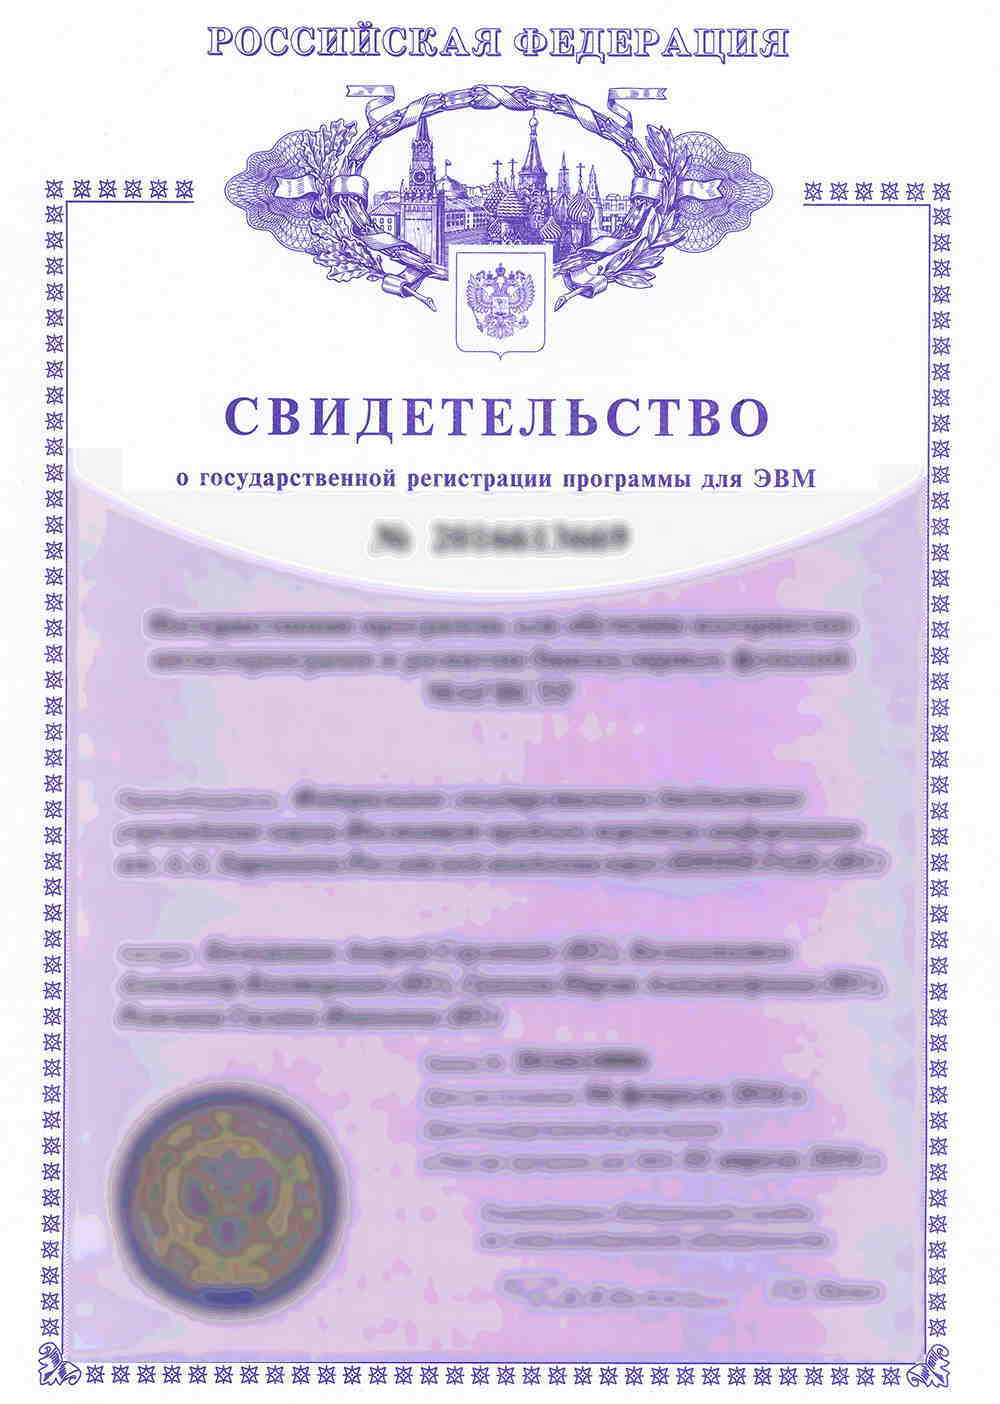
\includegraphics[width=0.98\textwidth]{svidetelstvo.jpg}


\end{document}
